\chapter{AI Scam szűrő API}

\section{Tanítási adatok felépítése}
\begin{flushleft}
    Maga a bemeneti fájl egy \verb|csv| kiterjesztésű fájl, mely tartalmaz \verb|Text| és \verb|Class| besorolásokat. A \verb|Text| besorolás jelzi az email üzenetet. A \verb|Class| besorolás pedig két értékkel bírhat: \verb|0| és \verb|1|. A \verb|0| érték jelzi, hogy az adott email üzenet nem veszélyes, csak egy általános email üzenet. \verb|1|-es érték jelzi a scam email üzenetet.
\end{flushleft}

\begin{flushleft}
    Fontossága a tanításnak, hogy maga az API képes legyen meghatározni, hogy majd a bejövő email üzenet káros-e vagy sem, ezáltal védi meg a felhasználót, hogy ne kattintson potenciális veszélyes email-re.
\end{flushleft}

\section{Modell}
\begin{flushleft}
    Konstruktoron belül, három teljesen összekapcsolt (lineáris) réteget határozunk meg. Ezek a rétegek felelősek a bemeneti adatok átalakításáért a megtanúlt súlyok segítségével:
    \begin{itemize}
        \item \textbf{self.fc1} $\rightarrow$ Az \verb|input_dim| dimenziójú bemenetet fogadja és 64 dimenziós kimenetet állít elő.
        \item \textbf{self.fc2} $\rightarrow$ Az \verb|fc1| kimenetét veszi (64 dimenzió) és egy 32 dimenziós kimenetet állít elő.
        \item \textbf{self.fc2} $\rightarrow$ Az \verb|fc2| kimenetét veszi (32 dimenzió) és létrehozza a 2 dimenziós végső kimenetet, amely két osztályt (0 és 1) képvisel.
    \end{itemize}
\end{flushleft}
\begin{listing}[H]
    \begin{minted}[linenos, numbersep=-10pt]{python3}
        import torch
        import torch.nn as nn

        class TextClassifier(nn.Module):
            def __init__(self, input_dim):
                super(TextClassifier, self).__init__()
                self.fc1 = nn.Linear(input_dim, 64)
                self.fc2 = nn.Linear(64, 32)
                self.fc3 = nn.Linear(32, 2)

            def forward(self, x):
                x = torch.relu(self.fc1(x))
                x = torch.relu(self.fc2(x))
                x = self.fc3(x)
                return x
    \end{minted}
    \caption{Szövegosztályozó modell}
    \label{code:modell}
\end{listing}

\newpage
\begin{flushleft}
    A \verb|forward| metódus meghatározza a neurális hálózat haladási irányát. Vár egy \verb|x| tenzor paramétert, és minden egyes definiált rétegnek átadja azt a \verb|rectified linear unit (ReLU)| aktiválás függvény (\verb|torch.relu|) segítségével. Ezután a végső eredményt adja vissza, ami a hálózat kimenete.
\end{flushleft}
\begin{listing}[H]
    \begin{minted}[linenos, numbersep=-10pt]{python3}
        def forward(self, x):
            x = torch.relu(self.fc1(x))
            x = torch.relu(self.fc2(x))
            x = self.fc3(x)
            return x
    \end{minted}
    \caption{Forward metódus}
    \label{code:forward}
\end{listing}

\begin{figure}[h]
    \centering
    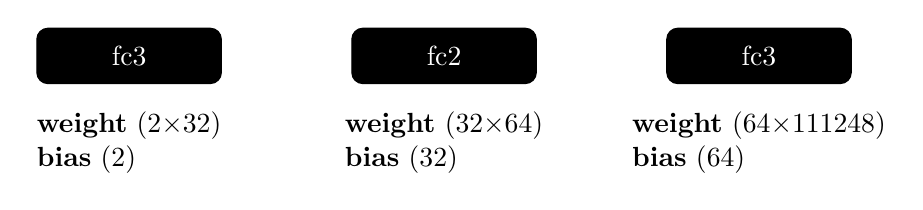
\begin{tikzpicture}[node distance=0.6cm, auto]
        % Define block styles
        \tikzstyle{block} = [rectangle, draw, fill=black, text=white, text width=6em, text centered, rounded corners, minimum height=2em]
        \tikzstyle{line} = [draw, -latex']
      
        % Place nodes
        \node [block] (header1) {fc3};
        \node [below of=header1, yshift=-0.5cm, align=left] (content1) {\textbf{weight} (2$\times$32)\\\textbf{bias} (2)};
      
        \node [block, right of=header1, node distance=4cm] (header2) {fc2};
        \node [below of=header2, yshift=-0.5cm, align=left] (content2) {\textbf{weight} (32$\times64$)\\\textbf{bias} (32)};
  
        \node [block, right of=header2, node distance=4cm] (header3) {fc3};
        \node [below of=header3, yshift=-0.5cm, align=left] (content3) {\textbf{weight} (64$\times111248$)\\\textbf{bias} (64)};
    \end{tikzpicture}
    \caption{Modell súlyok}
\end{figure}

\section{Tanítás}
\begin{flushleft}
    Először is beolvasásra kerülnek a tanítási adatok, melyek 'Text' és 'Class' értékekből állnak, így ezeket el kell szeparálni egymástól.
\end{flushleft}
\begin{listing}[H]
    \begin{minted}[linenos, numbersep=-10pt]{python3}
        data = pd.read_csv('fraud_email_.csv')

        data['Text'].fillna('', inplace=True)

        texts = data['Text'].tolist()
        labels = data['Class'].tolist()
    \end{minted}
    \caption{Tanítási adatok betöltése csv fájlból}
    \label{code:text_class}
\end{listing}

\newpage
\begin{flushleft}
    Létre kell hozni egy \verb|CountVectorizer()| példányt, mely szöveges dokumentumok gyűjteményét alakítja át mátrixba, ahol minden sor egy dokumentmot és minden oszlop egy egyedi szót a korpuszban reprezentál. Majd a \verb|fit_transform| metódus segítségével illesztjük a \verb|vectorizer|-t a megadott szöveges adathoz (\verb|texts|) és átalakítjuk a szöveges adatot egy mátrixba (\verb|X|).
\end{flushleft}
\begin{flushleft}
    Hogy később fel lehessen használni ezen adatokat a későbbiekben, szükséges menteni őket: \verb|count_vectorizer_vocab.pkl|; \verb|count_vectorizer.pkl| néven. A \verb|count_vectorizer_vocab.pkl| egy szótár, amely a szavakat indexeikkel társítja a mátrixban. A \verb|count_vectorizer.pkl| tartalmazza a szótárt és a hozzátartozó szükséges egyéb paramétereket/konfigurációkat.
\end{flushleft}
\begin{listing}[H]
    \begin{minted}[linenos, numbersep=-10pt]{python3}
        vectorizer = CountVectorizer()
        X = vectorizer.fit_transform(texts)

        with open('count_vectorizer_vocab.pkl', 'wb') as vocab_file:
            pickle.dump(vectorizer.vocabulary_, vocab_file)

        with open('count_vectorizer.pkl', 'wb') as vectorizer_file:
            pickle.dump(vectorizer, vectorizer_file)
    \end{minted}
    \caption{Beolvasott adatok előfeldolgozása}
    \label{code:data_pre}
\end{listing}

\begin{flushleft}
    Adatok konverzálása PyTorch tenzorokká, ahol először az \verb|X| változó kerül átalakításra a \verb|torch.tensor| segítségével. Így eredményül kapunk egy sűrűbb tenzort. Ezt követően a \verb|dtype=torch.float32| beállításával biztosítjuk, hogy a tenzor elemei lebegőpontos számok legyenek. Az \verb|y| változót is PyTorch tenzorrá alakítjuk, de \verb|int64| típust használunk, mert ezek a címkék osztályokat jelentenek.
\end{flushleft}
\begin{flushleft}
    Adatok felosztása tanító és teszt halmazokra a \verb|train_test_split| függvény segíttségével. Az \verb|X_train| és a \verb|y_train| változók tartalmazzák a tanító adathalmazt, míg az \verb|X_test| és \verb|y_test| változók a teszt adathalmazt. A \verb|test_size=0.2| azt jelenti, hogy a teszt halmaz a teljes adathalmaz 20\%-át fogja tartalmazni és a \verb|random_state=42| a véletlenszerűség vezérlésére szolgál, így az eredmények ismételhettőek lesznek.
\end{flushleft}
\begin{flushleft}
    Bemeneti dimenzió és modell létrehozása, ahol az \verb|input_dim| változóban eltároljuk a bemeneti dimenziót, ami a tanító adathalmazban lévő jellemzők számát jelenti. Ezután létrehozunk a már korábban létrehozott modellt (\verb|TextClassifier|) és átadjuk paraméterként a bemeneti dimenziót.
\end{flushleft}
\begin{listing}[H]
    \begin{minted}[linenos, numbersep=-10pt]{python3}
        X = torch.tensor(X.toarray(), dtype=torch.float32)
        y = torch.tensor(labels, dtype=torch.int64)

        X_train, X_test, y_train, y_test = train_test_split(X, y, test_size=0.2, random_state=42)

        input_dim = X_train.shape[1]
        model = TextClassifier(input_dim)
    \end{minted}
    \caption{PyTorch tenzorok}
    \label{code:pytensors}
\end{listing}

\newpage
\begin{flushleft}
    Először létrehozunk egy \verb|nn.CrossEntropyLoss| példányt, ami felel a veszteségekért. Azért került használatra, mert jól alkalmazható osztályozási problémákra, ahol az egyes példányok \underline{egyetlen helyes kategóriákhoz} tartoznak.
\end{flushleft}
\begin{flushleft}
    Az optimalizáló algoritmust az \verb|optim.Adam| osztály segítségével hozzuk létre. Az Adam egy hatékony optimalizáló algoritmus, amely alkalmazodik a tanítás során változó \verb|gradiens|hez \footnote{A gradiens egy vektor, amely tartalmazza egy függvény minden paraméterének parciális deriváltját egy adott pontban.}. A \verb|model.parameters()| az összes tanítható paramétert jelöli meg a modellben és ezeket fogja optimalizálni az algoritmus. Az \verb|lr=0.001| paraméter beállítja a tanulási ráta értékét, ami azt szabályozza, hogy mennyire legyenek nagyok a lépésközök a paraméterek frissítésekor.
\end{flushleft}
\begin{listing}[H]
    \begin{minted}[linenos, numbersep=-10pt]{python3}
        criterion = nn.CrossEntropyLoss()
        optimizer = optim.Adam(model.parameters(), lr=0.001)
    \end{minted}
    \caption{Vesztéség és optimalizáló algoritmus definiálása}
    \label{code:loss}
\end{listing}

\begin{flushleft}
    Maga a tanulási fázis egy cikluson keresztül megy végig (\verb|num_epochs|) és minden epoch kezdetén a gradiensek nullázódnak, hogy ne akkumulálódjanak az epochok között (\verb|optimizer.zero_grad()|). A modell előrejelzéseket hoz létre a tanító adathalmozon (\verb|outputs = model(X_train)|). A \verb|loss = criterion(outputs, y_train)| kiszámolja a veszteséget a modell előrejelzések és a valós címkék között a meghatározott veszteségfüggvény segítségével.
\end{flushleft}
\begin{flushleft}
    A \verb|loss.backward()| visszaterjeszti (backpropagation) a gradienseket a hálózaton, azaz kiszámolja a veszteségfüggvény parciális deriváltját a paraméterek szerint. Az \verb|optimizer.step()| optimalizációs algoritmus végrehajtja a paraméterek frissítését a tanító adathalmozon kiszámolt gradiensek alapján. Végül a veszteség értékét hozzáadjuk a \verb|train_losses| listához és elmentjük a tanítási eredményeket a \verb|spam_classifier_model.pth| néven.
\end{flushleft}
\begin{listing}[H]
    \begin{minted}[linenos, numbersep=-10pt]{python3}
        num_epochs = 20
        train_losses = []

        for epoch in range(num_epochs):
            optimizer.zero_grad()
            outputs = model(X_train)
            loss = criterion(outputs, y_train)
            loss.backward()
            optimizer.step()
            train_losses.append(loss.item())
            print(f'Epoch [{epoch + 1}/{num_epochs}], Loss: {loss.item():.4f}')

        torch.save(model.state_dict(), "spam_classifier_model.pth");
    \end{minted}
    \caption{Tanítási ciklus}
    \label{code:tloop}
\end{listing}

\newpage
\begin{flushleft}
    A \verb|torch.max| függvény segítségével megkeressük azokat a kimeneti oszlopokat, amelyekben a legnagyobb értékek vannak. A második visszatérési érték a maximális érték indexeit tartalmazza. Ezek az indexek az osztályokhoz tartozó előrejelzések.
\end{flushleft}
\begin{flushleft}
    A pontosság kiszámításánál az \verb|accuracy_score| felel. Tehát összehasonlítjuk a modell által előrejelzett osztályokat (\verb|predicted|) a valós osztályokkal (\verb|y_test|), majd kiszámoljuk a pontosságot.
\end{flushleft}
\begin{listing}[H]
    \begin{minted}[linenos, numbersep=-10pt]{python3}
        model.eval()
        with torch.no_grad():
            y_pred = model(X_test)
            _, predicted = torch.max(y_pred, 1)

        accuracy = accuracy_score(y_test.numpy(), predicted.numpy())
        print(f'Accuracy: {accuracy * 100:.2f}%')
    \end{minted}
    \caption{Modell kiértékelése}
    \label{code:eval}
\end{listing}

\section{Spam szűrése}
\begin{itemize}
    \item Végpont - \textbf{/spam-classification}
    \begin{itemize}
        \item \textbf{POST} (JSON)
    \end{itemize}
    \item Előfeltétel(ek): \textbf{Nincs}
\end{itemize}
\begin{itemize}
    \item Bemeneti paraméter(ek):
    \begin{itemize}
        \item text - Típus: \textbf{string}
    \end{itemize}
\end{itemize}
\begin{listing}[H]
    \begin{minted}[linenos, numbersep=-10pt]{json}
        {
            "text": "SAMPLE TEXT"
        }
    \end{minted}
    \caption{Példa adatok a spam üzenet szűrésére}
    \label{code:spam_filtering}
\end{listing}